\documentclass[a4paper,11pt,twocolumn,landscape]{article}

\usepackage{FabZ}
\usepackage{vecteurs}
\usepackage{repere}

\usepackage{geometry}
\geometry{hmargin=0.5cm,vmargin=1.5cm}

\newcommand{\milieu}[6]{$\pointcoord{A_{\theenumi}}{#1}{#2}$ et $\pointcoord{B_{\theenumi}}{#3}{#4}$ \hfill \reponseEX{$\pointcoord{M_{\theenumi}}{#5}{#6}$}}

\newcommand{\extremite}[6]{$\pointcoord{A_{\theenumi}}{#1}{#2}$ et $\pointcoord{M_{\theenumi}}{#3}{#4}$ \hfill \reponseEX{$\pointcoord{B_{\theenumi}}{#5}{#6}$}}

\newcommand{\longueur}[5]{$\pointcoord{A_{\theenumi}}{#1}{#2}$ et $\pointcoord{B_{\theenumi}}{#3}{#4}$ \hfill \reponseEX{Longueur $A_{\theenumi}B_{\theenumi}$ = $#5$}}

\newcommand{\quadrilatere}[9]{$\pointcoord{A_{\theenumi}}{#1}{#2}$, $\pointcoord{B_\theenumi}{#3}{#4}$ $\pointcoord{C_{\theenumi}}{#5}{#6}$, $\pointcoord{D_\theenumi}{#7}{#8}$ \\ \textcolor{red}{$A_{\theenumi}B_{\theenumi}C_{\theenumi}D_{\theenumi}$ est un #9.}}
%
%\setlength{\headheight}{0pt}
%\pagestyle{fancyplain}
%\fancyhf{}
%\lhead[]{\textbf{TD Vecteurs}}
%\chead[]{}
%\rhead[]{}
%
%\lfoot[]{}
%\cfoot[]{}
%\rfoot[]{}
%%\rfoot[]{Page \thepage~ sur \pageref{LastPage}}

\fancypagestyle{firststyle}
{
	\setlength{\headheight}{0em}
	\fancyhf{}
	\lhead[]{}
	\chead[]{\textbf{Repérage dans le plan}}
	\rhead[]{}

	\lfoot[]{}
	\cfoot[]{}
	\rfoot[]{}
%	\rfoot[]{Page \thepage~ sur \pageref{LastPage}}
}

\fancypagestyle{vide}
{
	\setlength{\headheight}{0em}
	\pagestyle{fancyplain}
	\def\headrulewidth{0em}
	\fancyhf{}
	\lhead[]{}
	\chead[]{}
	\rhead[]{}
	
	\lfoot[]{}
	\cfoot[]{}
	\rfoot[]{}
%	\rfoot[]{Page \thepage~ sur \pageref{LastPage}}
}

\usetikzlibrary{fadings}
\newcommand{\Fin}{node[xshift=-1.5ex,rotate=10]{F}
node[rotate=170]{i}
node[xshift=1.5ex,rotate=45]{n}}

\newcommand{\bonnesvacances}{node[xshift=0ex,rotate=10]{B}
node[xshift=1*1.5ex,rotate=170]{o}
node[xshift=2*1.5ex,rotate=45]{n}
node[xshift=3*1.5ex,rotate=128]{n}
node[xshift=4*1.5ex,rotate=75]{e}
node[xshift=5*1.5ex,rotate=130]{s}
node[xshift=6*1.5ex,rotate=85]{~}
node[xshift=7*1.5ex,rotate=128]{v}
node[xshift=8*1.5ex,rotate=43]{a}
node[xshift=9*1.5ex,rotate=4]{c}
node[xshift=10*1.5ex,rotate=145]{a}
node[xshift=11*1.5ex,rotate=5]{n}
node[xshift=12*1.5ex,rotate=25]{c}
node[xshift=13*1.5ex,rotate=105]{e}
node[xshift=14*1.5ex,rotate=45]{s}
}


\begin{document}
\begin{minipage}{0.45\textwidth}
\thispagestyle{firststyle}

\paragraph*{Exercice 1}~\\

\begin{minipage}{0.5\textwidth}
\begin{center}
%\fbox{
\begin{tikzpicture}[scale=1.8,every node/.style={scale=0.7}]
	%Points
	\coordinate(A)at(-1,0);
	\coordinate(B)at(-1,-1);
	\coordinate(C)at(0,-1);
	\coordinate(D)at(0,0);
	\coordinate(E)at(0,1);
	\coordinate(F)at(-1,1);
	\coordinate(G)at(1,0);
	\coordinate(H)at(1,1);
	\coordinate(I)at(2,0);
	\coordinate(J)at(-1,2);
	\draw (A)--(B)--(C)--(D)--cycle;
	\draw (A)--(D)--(E)--(F)--cycle;
	\draw (D)--(G)--(H)--(E)--cycle;
	\draw (F)--(J);
	\draw (C)--(G);
	\draw (G)--(I);
	\draw (H)--(I);
	%Étiquettes
	\foreach \point in {A, ..., G, I, J}
		\draw(\point)node{$\times$};
	\foreach \point in {A, ..., G, I, J}
		\draw(\point)node[below right]{$\point$};
	\foreach \point in {H}
		\draw(\point)node{$\times$};
	\foreach \point in {H}
		\draw(\point)node[above right]{$\point$};
\end{tikzpicture}
%}
\end{center}
\end{minipage}
\begin{minipage}{0.5\textwidth}
$BCDA$, $ADEF$ et $DGHE$ sont des carrés de côté $1$.
~\\~\\
De plus le point $I$ est sur la droite $(AG)$ avec $GI = 1$ et le point $J$ sur la droite $(BF)$ avec $FJ = 1$.

\end{minipage}

\vspace*{2em}

\begin{enumerate}
	\item Déterminer les coordonnées de tous les points de la figure
	\begin{enumerate}
		\item dans le repère $(D, G, E)$ qui est orthonormé.
		\item dans le repère $(A, G, J)$ qui est aussi orthonormé.
	\end{enumerate}
~\\
\textbf{A partir de maintenant on n’utilisera que le repère $\mathbf{\left(D, G, E\right)}$.}

	\item Déterminer dans ce repère les coordonnées des points
	\begin{enumerate}
		\item $K$ milieu de $\left[CI\right]$
		\item $L$ milieu de $\left[HJ\right]$.
	\end{enumerate}

	\item Le quadrilatère $FLIK$ est-il un parallélogramme ? Justifier.

	\item Déterminer les coordonnées des points
	\begin{enumerate}
		\item $M$ milieu de $\left[AL\right]$
		\item $N$ milieu de $\left[GI\right]$.
	\end{enumerate}
	Le quadrilatère MLNK est-il un parallélogramme ? Justifier.
	\item Déterminer les coordonnées du point $P$ milieu de $\left[FN\right]$ puis du point $O$ tel que $FLNO$ soit un parallélogramme.
	\item Calculer les longueurs des diagonales $FN$ et $LO$ de ce parallélogramme.
	\item Le triangle $FLK$ est-il rectangle ?
	\item Les points $A$, $O$, $G$ et $H$ sont-ils situés sur un même cercle ?
\end{enumerate}

\vspace{-2em}


\end{minipage}
\newpage
\begin{minipage}{0.45\textwidth}
\thispagestyle{firststyle}

\paragraph*{Exercice 2}~\\

\begin{minipage}{0.5\textwidth}
\begin{center}
%\fbox{
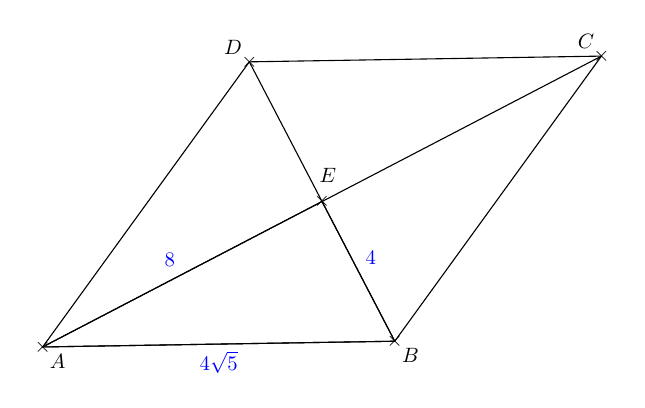
\begin{tikzpicture}[scale=0.5,every node/.style={scale=0.75}]
	%Points
	\begin{scope}[rotate=-62.5]
	\coordinate(A)at(0,0);
	\coordinate(B)at(4,8);
	\coordinate(C)at(0,16);
	\coordinate(D)at(-4,8);
	\coordinate(E)at(0,8);
%	\coordinate(F)at(-1,1);
%	\coordinate(G)at(1,0);
%	\coordinate(H)at(1,1);
%	\coordinate(I)at(2,0);
%	\coordinate(J)at(-1,2);
	\draw (A)--(B)--(C)--(D)--cycle;
	\draw (A)--(C);
	\draw (B)--(D);
	\draw (A)--(E) node[midway, above left, blue]{$8$};
	\draw (B)--(E) node[midway, above right, blue]{$4$};
	\draw (A)--(B) node[midway, below, blue]{$4\sqrt{5}$};
	%Étiquettes
	\foreach \point in {A, B}
		\draw(\point)node{$\times$};
	\foreach \point in {A, B}
		\draw(\point)node[below right]{$\point$};
	\foreach \point in {E}
		\draw(\point)node{$\times$};
	\foreach \point in {E}
		\draw(\point)node[above,shift={(0.1,0.2)}]{$\point$};
	\foreach \point in {C, D}
		\draw(\point)node{$\times$};
	\foreach \point in {C, D}
		\draw(\point)node[above left]{$\point$};
%	\foreach \point in {H}
%		\draw(\point)node{$\times$};
%	\foreach \point in {H}
%		\draw(\point)node[above right]{$\point$};
	\end{scope}
\end{tikzpicture}
%}
\end{center}
\end{minipage}
\begin{minipage}{0.5\textwidth}
Le parallélogramme ci-contre est-il un losange~?
\end{minipage}

\vspace*{2em}

\paragraph*{Exercice 3}~\\


$ABC$ est un triangle isocèle en $A$. Le cercle $\mathscr{C}$ , de diamètre $[AB]$, coupe $[BC]$ en $D$ et $[AC]$ en $E$. La perpendiculaire à $(AB)$ passant par $C$ coupe la droite $(BE)$ en $F$.

\textbf{Objectif :} Démontrer que $A$, $D$ et $F$ sont alignés, et que $(AF)$ est la médiatrice de $[BC]$.
\begin{enumerate}
	\item Faire une figure.
	\item	\begin{enumerate} 
				\item Quelle est la nature des triangles $AEB$ et $ADB$~?
				\item Pourquoi peut-on affirmer que $F$ est l’orthocentre du triangle $ABC$~?
				\item Pourquoi peut-on affirmer que $(AD)$ est la médiatrice de $[BC]$~?
			\end{enumerate}
	\item	\begin{enumerate} 
				\item Montrer que $(AF)$ et $(BC)$ sont perpendiculaires.
				\item En déduire que $A$, $D$, et $F$ sont alignés, puis que $(AF)$ est médiatrice de $[BC]$.
			\end{enumerate}
\end{enumerate}

\paragraph*{Exercice 4}~\\

Les diagonales d’un quadrilatère $ABCD$ se coupent en $E$.

$I$, $J$, $K$, $L$ sont les milieux respectifs de $[AB]$, $[BC]$, $[CD]$, $[DA]$.

\begin{enumerate}
	\item Faire une figure en y reportant toutes les informations de l’énoncé.
	\item Démontrer que $IJKL$ est un parallélogramme.
\end{enumerate}


%
%\begin{enumerate}
%	\item Déterminer les coordonnées de tous les points de la figure
%	\begin{enumerate}
%		\item dans le repère $(D, G, E)$ qui est orthonormé.
%		\item dans le repère $(A, G, J)$ qui est aussi orthonormé.
%	\end{enumerate}
%~\\
%\textbf{A partir de maintenant on n’utilisera que le repère $\mathbf{\left(D, G, E\right)}$.}
%
%	\item Déterminer dans ce repère les coordonnées des points
%	\begin{enumerate}
%		\item $K$ milieu de $\left[CI\right]$
%		\item $L$ milieu de $\left[HJ\right]$.
%	\end{enumerate}
%
%	\item Le quadrilatère $FLIK$ est-il un parallélogramme ? Justifier.
%
%	\item Déterminer les coordonnées des points
%	\begin{enumerate}
%		\item $M$ milieu de $\left[AL\right]$
%		\item $N$ milieu de $\left[GI\right]$.
%	\end{enumerate}
%	Le quadrilatère MLNK est-il un parallélogramme ? Justifier.
%	\item Déterminer les coordonnées du point $P$ milieu de $\left[FN\right]$ puis du point $O$ tel que $FLNO$ soit un parallélogramme.
%	\item Calculer les longueurs des diagonales $FN$ et $LO$ de ce parallélogramme.
%	\item Le triangle $FLK$ est-il rectangle ?
%	\item Les points $A$, $O$, $G$ et $H$ sont-ils situés sur un même cercle ?
%\end{enumerate}

\vspace{-2em}

\end{minipage}

\end{document}
%
%
%\paragraph{Exercice~2} Propriétés des quadrilatères
%
%\begin{tikzpicture}[scale=1,every node/.style={scale=0.7}]
%\tikzstyle{debutfin}=[ellipse,draw,text=red]
%\tikzstyle{instruct}=[rectangle,draw,fill=yellow!50]
%\tikzstyle{test}=[diamond, aspect=6,thick,
%draw=blue,fill=yellow!50,text=blue]
%\tikzstyle{es}=[rectangle,draw,rounded corners=4pt,fill=blue!25]
%
%\node[debutfin] (debut) at (0,3) {Début};
%\node[es] (lire) at (0,2) {Prendre un quadrilatère $Q$};
%\node[test] (test) at (0,0) {Les diagonales ont-elles un milieu commun \ ?};
%%\node[instruct] (init) at (-2,2.5) {$S\leftarrow 0$};
%\node[instruct] (plus) at (0,-2.5) {$S\leftarrow S+N$};
%\node[instruct] (moins) at (0,-3.5) {$N\leftarrow N-1$};
%\node[es] (afficher) at (-4,-2) {Afficher la somme $S$};
%\node[debutfin] (fin) at (-4,-3) {Fin};
%
%\tikzstyle{suite}=[->,>=stealth,thick,rounded corners=4pt]
%\draw[suite](debut) -- (lire);
%\draw[suite](lire) -- (test.north);
%%\draw[suite](init) -- (test.north);
%\draw[suite](test.south) -- (plus);
%\draw[suite](plus) -- (moins);
%\draw[suite](test) -| (afficher);
%\draw[suite](afficher) -- (fin);
%\end{tikzpicture}
%
%
%%%%%\begin{tikzpicture}
%%%%%% définition des styles
%%%%%\tikzstyle{quadri}=[rectangle,draw,fill=yellow!50,text=blue]
%%%%%\tikzstyle{estun}=[->,>=latex,very thick,dotted]
%%%%%% les nœuds
%%%%%\node[quadri] (Q) at (0,3) {Quadrilatère};
%%%%%\node[quadri] (P) at (0,1.5) {Parallélogramme};
%%%%%\node[quadri] (R) at (-3,0) {Rectangle};
%%%%%\node[quadri] (L) at (3,0) {Losange};
%%%%%\node[quadri] (C) at (5,-1.5) {Carré};
%%%%%% les flèches
%%%%%\draw[estun] (P)--(Q);
%%%%%\draw[estun] (R)to[bend left](Q); \draw[estun] (R)--(P);
%%%%%\draw[estun] (L)--(Q.south east); \draw[estun] (L)--(P);
%%%%%\draw[estun] (C)to[bend right](Q.east); \draw[estun] (C)to[bend left](P);
%%%%%\draw[estun] (C)--(L.south east); \draw[estun] (C)to[bend left](R);
%%%%%% la légende
%%%%%\draw[estun] (-4.5,2.5)--(-3,2.5)node[midway,above]{est un};
%%%%%\end{tikzpicture}